\section{Commutazione}
    Come ormai sappiamo bene, una rete è un insieme di dispositivi connessi tra di loro in base alla topologia adottata (nella topologia mesh, canale punto-punto per ogni coppia di dispositivi; in alternativa, nella topologia a stella, vi è un nodo centrale e un canale fra tale nodo e ogni altro dispositivo). 
    
    La connessione è tale da connettere \textit{ogni} coppia di dispositivi. Nella realtà, quest'idea non è praticabile. Il numero e la lunghezza dei collegamenti costituirebbero costi troppi elevati. La soluzione è lo \textbf{switching}, cioè la commutazione.
    
    \vspace{3mm}
    
    Per connettere un insieme di nodi terminali (\textit{stazioni}), vengono utilizzati dei \textbf{nodi speciali interconnessi} (\textit{switch}), cioè dei dispositivi capaci di \textbf{creare connessioni temporanee} fra due o più stazioni connesse agli switch. Il loro utilizzo è limitato alla creazione di connessioni temporanee. Uno switch ha varie modalità di funzionamento, dette \textbf{commutazioni}. 
    
    Fondamentalmente, gli switch creano percorsi fra due nodi terminali.
    
    \subsection{Categorie di commutazione}
    
        Le \textit{categorie di commutazioni} sono:
        
        \begin{itemize}
            \item 
                Reti a commutazione
            
            \begin{itemize}
                \item 
                    Reti a commutazione di circuito
                    
                \item 
                    Reti a commutazione di messaggio
    
                \item 
                    Reti a commutazione di pacchetto
                
                    \begin{itemize}
                        \item 
                            Reti a datagram
                            
                        \item 
                            Reti a circuito virtuale
                    \end{itemize}
            \end{itemize}
        \end{itemize}
    
        \subsubsection{Commutazione di circuito}
                    
            La commutazione avviene nello \textbf{strato fisico}.
                
            Un nodo vuole inviare informazioni ad un altro nodo della rete. Prima di iniziare la comunicazione, le stazioni (nodi) devono effettuare una prenotazione delle risorse necessarie per la comunicazione. \textbf{Gli switch prenotano le risorse e definiscono il percorso}; tali risorse devono rimanere dedicate a questa connessione per tutta la durata del trasferimento dei dati, fino alla fase di eliminazione del circuito.
                
            \vspace{3mm}    
            
            I dati trasferiti tra due stazioni non sono scomposti in pacchetti, ma spediti in un flusso continuo dalla stazione mittente a quella destinataria.
                
            Inoltre, non c'è bisogno di indirizzamento durante il trasferimento dei dati dato che il circuito viene attribuito a priori. Gli switch instradano i dati in base al canale riservato nella fase di instaurazione del circuito. Il vantaggio della commutazione di circuito giace nell'assenza di tempo di attesa negli switch.

            \vspace{3mm}
            
            I problemi principali delle reti a commutazione di circuito sono la scarsa efficienza dovuta al ritardo di rete e ad un generale ritardo dovuto al tempo necessario ad instaurare il circuito, trasferire i dati ed eliminare il circuito. Il ritardo coincide con la somma fra tempo di propagazione della richiesta della stazione sorgente, il tempo necessario a trasferire la richiesta, il tempo di propagazione della risposta della stazione destinataria e il tempo per trasferire la risposta.

            \vspace{3mm}

            \textbf{Esempio tipico di commutazione di circuito}
                
            \begin{center}
                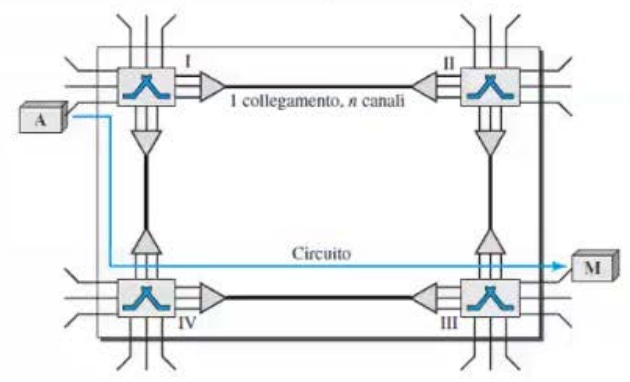
\includegraphics[scale=0.75]{images/Circuito_Fase1.png}
            \end{center}
                
            \textbf{Fase I - Instaurazione della connessione}
                
            \vspace{3mm}
                
            \textit{Fase I.A - Obiettivo:} $A$ spedisce una richiesta all'indirizzo $M$.
                
            \begin{itemize}
            
                \item
                    $A$ spedisce la richiesta allo switch $I$ con l'indirizzo di $M$.
                    
                \item
                    $I$ spedisce la richiesta allo switch $IV$.
                    
                \item
                    $IV$ spedisce la richiesta allo switch $III$.
                    
                \item
                    $III$ spedisce la richiesta ad $M$.
                    
            \end{itemize}
            
            \textit{Fase I.B - Obiettivo:} $M$ accetta la richiesta
            
            \vspace{3mm}
            
            $M$ risponde a $III$, che risponde a $IV$, che risponde a $I$, che risponde ad $A$.
            
            \vspace{3mm}
            
            \textbf{Fase II - Spedizione dei dati}
            
            \vspace{3mm}
            
            $A$ spedisce i dati indicando il circuito instaurato nella prima fase. Adesso, gli switch conoscono la posizione di $M$ e sanno che i dati devono arrivare lì, partendo da $A$, sfruttando il canale dedicati ai dati.
            
            \vspace{3mm}
            
            \textbf{Fase III - Chiusura della connessione}
            
            \vspace{3mm}
            
            \textit{ Fase III.A - Obiettivo:} $A$ chiude la connessione.
            
            \begin{itemize}
                \item 
                    $A$ spedisce la richiesta di chiusura allo switch $I$
                
                \item
                    $I$ libera le risorse riservate
                    
                \item
                    $I$ spedisce la richiesta di chiusura allo switch $IV$
                    
                \item
                    $IV$ libera le risorse riservate
                    
                \item
                    $IV$ spedisce la richiesta di chiusura allo switch $III$
                    
                \item
                    $III$ libera le risorse riservate
                    
                \item
                    $III$ spedisce la richiesta di chiusura a $M$
            \end{itemize}
            
            Il \textit{tempo necessario} ad inviare dati lungo una rete a commutazione di circuito è la somma del tempo necessario a svolgere le tre fasi sopraelencate. 
            
            Il \textit{ritardo}, invece, è la somma del tempo di propagazionme della richiesta della stazione sorgente, del tempo necessario a trasferire la richiesta, del tempo di propagazione della risposta della stazione destinatario e del tempo per trasferire la risposta.
            
        \subsubsection{Commutazione di pacchetto}
        
            I messaggi devono essere divisi in pacchetti, detti \textbf{datagram}, a lunghezza variabile o fissa. Si smistano i pacchetti lungo la rete in maniera ottimale.
            
            La grandezza dei pacchetti è determinata dalla rete e dal protocollo che ne gestisce il funzionamento. Non c'è allocazione di risorse per un pacchetto; non ci sono canali riservati, né risorse riservate negli switch. I pacchetti sono gestiti tramite FIFO.
            
            \vspace{3mm}
            
            I pacchetti vengono instradati verso la loro destinazione tramite le \textbf{tavole di routing}, che contiene informazioni di instradamento in funzione dell'indirizzo di destinazione. Gli switch, dunque, sono dotati di queste tavole di routing.
            
            \vspace{3mm}
            
            I ritardi di una rete a datagram possono essere maggiori di quelli in una rete a circuito. Ogni pacchetto potrebbe subire un significativo ritardo su ogni switch prima di essere inoltrato. Chiaramente, questo dipende dalla grandezza della struttura di tipo FIFO.
            
        \subsubsection{Commutazione a circuito virtuale}
        
            Sono una via di mezzo fra la commutazione di circuito e la commutazione di datagram e sintetizza le caratteristiche di entrambe.
            
            I dati sono divisi in pacchetti, ogni pacchetto contiene un indirizzo di destinazione. Le risorse necessarie possono essere allocate dinamicamente.
            
            \vspace{3mm}
            
            Analogamente alle reti a commutazione di circuito, inoltre, vi è una fase di instaurazione (in cui uno switch crea una riga nella tavola di routing per il circuito virtuale dela connessione richiesta) e di chiusura della connessione, oltre al trasferimento dei dati. 
            
            Tutti i pacchetti seguono lo stesso percorso, stabilito durante la connessione. Le risorse necessarie sono prenotate, come nella commutazione di circuito. E' implementata nello strato di collegamento, fisico e di rete.
            
            \begin{center}
                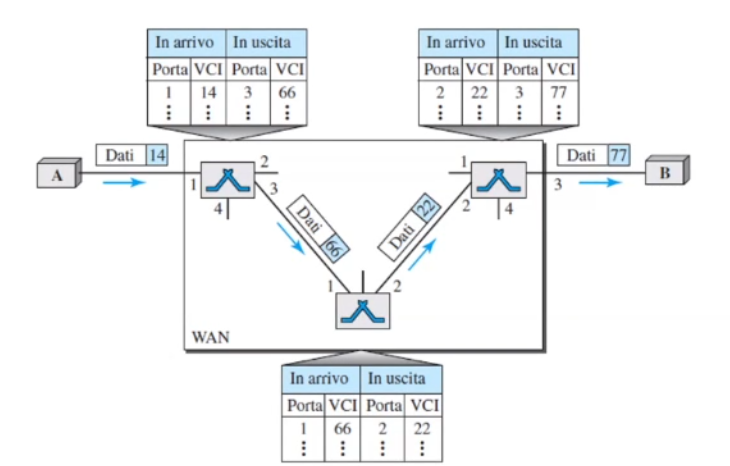
\includegraphics[scale=0.5]{images/Tavola-di-Routing.png}
            \end{center}
            
            \vspace{3mm}
            
            Utilizza due tipi di instradamento: \textit{globale} (qualsiasi nodo della rete deve avere un indirizzo globale) e \textit{locale} (degli identificatori di circuito virtuali - VCI - vengono usati per trasferire dati; i VCI sono numeri con significati locali, in base alla coppia di switch: in pratica, combina switch a switch).
            
    \subsection{Struttura dello switch}
    
        La tecnologia attuale per gli switch di una rete a circuito virtuale utilizza \textbf{switch a divisione di spazio} (crossbar, switch a più livelli) e \textbf{switch a divisione di tempo}.
        
        \vspace{3mm}
        
        Negli \textbf{switch a divisione di spazio}, i circuiti sono separati fisicamente. Ogni switch occupa il proprio spazio, e originariamente furono progettati per reti analogiche. 
        
        Gli switch a \textit{crossbar} dispongono $n$ linee di input verso $m$ linee di output. I punti di incrocio sono $n*m$. Gli switch \textit{a più livelli} combinano vari switch crossbar a più livelli, appunto. Il vantaggio degli switch a divisione di spazio è la comunicazione istantanea; lo svantaggio è il numero di punti di incrocio necessari affinché lo switch non sia bloccante.
        
        \vspace{3mm}
        
        Gli \textbf{switch a divisione di tempo} utilizzano il TDM con tecnologia a scambio di intervalli temporali (TSI). Il vantaggio degli switch a divisione di tempo è che non richiede punti di incrocio; lo svantaggio è che la gestione di ogni connessione crea ritardi.
        
        \vspace{3mm}
        
        Infine, gli \textbf{switch misti} combinano gli switch a divisione di spazio e divisione di tempo.